% =============================================================================
%                    WEEK 5: COOPERATIVE GAMES (PART II)
% =============================================================================
\section{Week 5: Cooperative Games (Part II)}

% -----------------------------------------------------------------------------
%                              5.1 TOPIC SUMMARY
% -----------------------------------------------------------------------------
\subsection{Topic Summary}

\begin{keybox}[Learning Objectives]
By the end of this week, you will be able to:
\begin{enumerate}
  \item Describe the core concepts of \textbf{hedonic games}, including non-transferable utility, preferences over coalitions, and compact representations.
  \item Model coalition formation problems using \textbf{additively separable hedonic games} (ASHGs) and related classes.
  \item Analyse stability concepts for hedonic games: \textbf{individual rationality}, \textbf{Nash stability}, \textbf{individual stability}, \textbf{contractual individual stability}, and \textbf{core stability}.
  \item Describe the \textbf{stable matching problem}, including preference profiles, stability, and blocking pairs.
  \item Apply the \textbf{Gale-Shapley deferred acceptance algorithm} to find stable matchings in bipartite settings.
  \item Prove key properties of DA: termination, perfection, stability, man-optimality, women-pessimality.
  \item Evaluate fairness and strategic aspects of stable matchings, including strategyproofness.
  \item Interpret applications of stable matching theory (college admissions, medical residencies, school choice).
\end{enumerate}
\end{keybox}

\separator

\subsubsection*{The Big Picture}

Week~4 covered \textbf{transferable utility} (TU) games where coalitions split a shared surplus. This week moves to \textbf{non-transferable utility} (NTU) settings where payoffs accrue directly to individuals and cannot be redistributed. The central model is the \textbf{hedonic game}, where each player's utility depends only on the composition of their coalition.

The second half introduces the \textbf{stable matching problem}---a special hedonic game where agents from two sides (e.g.\ men/women, students/hospitals) must be paired. The \textbf{Gale-Shapley algorithm} always finds a stable matching, and its properties (optimality, pessimality, strategyproofness) have profound practical consequences.

\separator

\subsubsection*{What Examiners Like to Ask}

\begin{itemize}
  \item Given an ASHG with a parameter, determine for which values a coalition structure is \textbf{individually rational}, \textbf{Nash stable}, or \textbf{in the core}.
  \item State the hierarchy of stability concepts and give examples where one holds but a stronger one fails.
  \item Trace the \textbf{Gale-Shapley algorithm} on a given preference instance step-by-step.
  \item Construct worst-case instances where DA requires many proposals.
  \item Explain why DA is \textbf{man-optimal} and \textbf{women-pessimal}; reproduce the proof.
  \item Determine whether DA is \textbf{strategyproof} for men, women, or both.
  \item Give an instance of the \textbf{stable roommate problem} with no stable matching.
  \item Describe extensions: many-to-one matching, unacceptable pairs, indifferences.
\end{itemize}

\separator

% -----------------------------------------------------------------------------
%           5.2 OVERVIEW + CORE CONCEPTS + EXTENDED THEORY
% -----------------------------------------------------------------------------
\subsection{Overview + Core Concepts + Extended Theory}

\subsubsection*{Roadmap}
\begin{enumerate}
  \item Non-transferable utility (NTU) games and hedonic games
  \item Compact representations: ASHGs, fractional, B-games, W-games
  \item Stability concepts: IR, Nash, individual, CIS, core
  \item Friends-and-enemies games
  \item Stable matching problem: formal model
  \item Gale-Shapley deferred acceptance algorithm
  \item Properties: termination, perfection, stability, optimality
  \item Strategyproofness
  \item Extensions and applications
\end{enumerate}

\bigseparator

% --- NTU and Hedonic Games ---
\subsubsection{Non-Transferable Utility Games}

\begin{defbox}[NTU Games]
In \textbf{non-transferable utility games}:
\begin{itemize}
  \item Payoffs accrue to \textbf{individual} coalition members and \textbf{cannot be transferred}.
  \item A coalition may have \textbf{multiple actions} producing different payoff vectors for its members.
  \item Example: coalition $\{x, y\}$ can perform action $a$ (payoffs $1, 6$) or action $b$ (payoffs $4, 2$).
\end{itemize}

\textbf{Motivating example:} $n$ researchers at different universities form groups to write papers. Each author receives rewards from their own university (promotion, bonus, teaching reduction)---these are \textbf{non-transferable}.
\end{defbox}

\separator

\subsubsection{Hedonic Games}

\begin{defbox}[Hedonic Game]
A \textbf{hedonic game} is a pair $(N, (\succeq_i)_{i \in N})$ where:
\begin{itemize}
  \item $N = \{1, \ldots, n\}$ is a set of \textbf{players}
  \item Each player $i$ has a preference relation $\succeq_i$ over $\{S \subseteq N \mid i \in S\}$ (all coalitions containing $i$)
  \item The outcome is a \textbf{coalition structure} (partition of $N$)---no payoff distribution phase
  \item Player $i$'s utility depends \textbf{only} on the coalition $i$ belongs to
\end{itemize}

Special case of NTU games: each coalition has only \textbf{one action} available (forming itself).
\end{defbox}

\begin{exbox}[Hedonic Game Example]
Three players with preferences:
\begin{itemize}
  \item 1: $\{1, 2\} \sim \{1, 3\} \succ \{1, 2, 3\} \succ \{1\}$
  \item 2: $\{2\} \succ \{1, 2, 3\} \succ \{1, 2\} \succ \{2, 3\}$
  \item 3: $\{1, 2, 3\} \succ \{3\} \succ \{2, 3\} \sim \{1, 3\}$
\end{itemize}

Preferences can be encoded numerically: e.g.\ $v_1(\{1,2\}) = v_1(\{1,3\}) = 2$, $v_1(\{1,2,3\}) = 1$, $v_1(\{1\}) = 0$.
\end{exbox}

\separator

\subsubsection{Compactly Representable Hedonic Games}

Full hedonic preferences are exponential in $n$. Several compact representations exist:

\begin{defbox}[Compact Representations]
Each agent $i$ assigns a value $v_i(j)$ to every other agent $j \in N \setminus \{i\}$:

\begin{center}
\renewcommand{\arraystretch}{1.4}
\begin{tabular}{@{} l p{8cm} @{}}
\toprule
\textbf{Class} & \textbf{Utility of $i$ in coalition $S$} \\
\midrule
\textbf{Additively Separable (ASHG)} & $v_i(S) = \displaystyle\sum_{j \in S \setminus \{i\}} v_i(j)$ \\[6pt]
\textbf{Fractional} & $v_i(S) = \dfrac{\sum_{j \in S \setminus \{i\}} v_i(j)}{|S|}$ \\[6pt]
\textbf{B-game (Best)} & $v_i(S) = \displaystyle\max_{j \in S \setminus \{i\}} v_i(j)$ \\[6pt]
\textbf{W-game (Worst)} & $v_i(S) = \displaystyle\min_{j \in S \setminus \{i\}} v_i(j)$ \\
\bottomrule
\end{tabular}
\end{center}

Also: \textbf{anonymous games} where preferences depend on coalition size only.
\end{defbox}

\begin{defbox}[ASHGs vs.\ Induced Subgraph Games]
Both use a weighted graph representation (players = vertices):
\begin{center}
\renewcommand{\arraystretch}{1.3}
\begin{tabular}{@{} l p{5cm} p{5cm} @{}}
\toprule
 & \textbf{Induced Subgraph Games} & \textbf{ASHGs} \\
\midrule
Edges & Undirected & Directed \\
Value of coalition $T$ & Total weight of internal edges & Sum of $i$'s outgoing edges to $T \setminus \{i\}$ \\
Symmetry & Always symmetric & Not necessarily \\
\bottomrule
\end{tabular}
\end{center}
\end{defbox}

\bigseparator

% --- Stability Concepts ---
\subsubsection{Stability Concepts for Hedonic Games}

The stability concepts form a hierarchy (strongest to weakest):
\[
\text{Core stable} \;\Rightarrow\; \text{Nash stable} \;\Rightarrow\; \text{Individually stable} \;\Rightarrow\; \text{CIS} \;\Leftarrow\; \text{(always exists)}
\]
Also: Nash stable $\Rightarrow$ Individually rational.

\begin{defbox}[Individual Rationality (IR)]
A partition is \textbf{individually rational} if no player strictly prefers being alone:
\[
v_i(S_i) \geq v_i(\{i\}) \quad \text{for all } i \in N
\]
where $S_i$ is $i$'s coalition in the partition. This is the \textbf{minimum stability requirement}.
\end{defbox}

\begin{defbox}[Nash Stability (NS)]
Player $i$ has an \textbf{NS-deviation} from partition $P$ if there exists $T \in P \cup \{\emptyset\}$ such that $i$ prefers $T \cup \{i\}$ to their current coalition.

A partition is \textbf{Nash stable} if no player has an NS-deviation.

\textbf{Key:} Player $i$ can move unilaterally to any existing coalition (or form a singleton)---\textbf{no consent needed} from the receiving coalition.
\end{defbox}

\begin{thmbox}[Nash Stability May Not Exist]
There exists a two-player game with no Nash stable outcome: if the red player values the yellow player positively but yellow values red negatively, then $\{\{r,y\}\}$ is unstable (yellow deviates) and $\{\{r\},\{y\}\}$ is unstable (red deviates).
\end{thmbox}

\begin{thmbox}[Nash Stability in Symmetric ASHGs]
In \textbf{symmetric ASHGs} ($v_i(j) = v_j(i)$ for all $i, j$):
\begin{itemize}
  \item Every such game admits a Nash stable outcome.
  \item Every NS-deviation increases the sum of utilities (social welfare).
  \item Finding a Nash stable outcome is \textbf{PLS-complete} (Gairing, Savani '10).
\end{itemize}
\end{thmbox}

\begin{defbox}[Individual Stability (IS)]
Player $i$ has an \textbf{IS-deviation} from partition $P$ if there exists $T \in P \cup \{\emptyset\}$ such that:
\begin{enumerate}
  \item $i$ prefers $T \cup \{i\}$ to their current coalition, \textbf{and}
  \item all players in $T$ \textbf{weakly prefer} $T \cup \{i\}$ to $T$.
\end{enumerate}

Compared to NS: the receiving coalition must \textbf{approve} the newcomer.
\end{defbox}

\begin{defbox}[Contractual Individual Stability (CIS)]
Player $i$ has a \textbf{CIS-deviation} from partition $P$ if there exists $T \in P \cup \{\emptyset\}$ such that:
\begin{enumerate}
  \item $i$ prefers $T \cup \{i\}$ to their current coalition $S$
  \item All players in $T$ weakly prefer $T \cup \{i\}$ to $T$ \quad (receiving coalition approves)
  \item All players in $S$ weakly prefer $S \setminus \{i\}$ to $S$ \quad (leaving coalition approves)
\end{enumerate}
\end{defbox}

\begin{thmbox}[Every Hedonic Game Has a CIS Outcome]
\textbf{Proof:}
\begin{enumerate}
  \item Encode preferences numerically (always possible).
  \item Every CIS-deviation \textbf{increases} the sum of utilities across all agents.
  \item A partition that \textbf{maximises} the sum of utilities must be CIS (no improving deviation exists). \qed
\end{enumerate}
\end{thmbox}

\begin{defbox}[Core Stability]
A group $C \subseteq N$ \textbf{blocks} a partition $P$ if every player in $C$ prefers $C$ to their coalition in $P$.

A partition is \textbf{core stable} if no group blocks it.
\end{defbox}

\begin{exbox}[Empty Core in a Hedonic Game]
Three players:
\begin{itemize}
  \item 1: $\{1, 2\} \succ \{1, 3\} \succ \{1\} \succ \{1, 2, 3\}$
  \item 2: $\{2, 3\} \succ \{2, 1\} \succ \{2\} \succ \{1, 2, 3\}$
  \item 3: $\{3, 1\} \succ \{3, 2\} \succ \{3\} \succ \{1, 2, 3\}$
\end{itemize}

\textbf{Analysis:} Grand coalition is blocked (any singleton prefers to leave). Singletons are blocked (any pair prefers to form). Any pair $\{i,j\}$ is blocked: the non-favourite member of the pair prefers to leave and join the singleton. The core is \textbf{empty}.
\end{exbox}

\begin{thmbox}[Core of ASHGs]
\begin{itemize}
  \item The core may be empty even for \textbf{symmetric} ASHGs (5-player counterexample with negative weights: no coalition of size $\geq 3$ is IR; no partition into singletons and pairs is stable).
  \item If all edge weights are \textbf{non-negative}, the grand coalition is core stable (trivially: every agent's utility is maximised).
\end{itemize}
\end{thmbox}

\separator

\subsubsection{Friends-and-Enemies Games}

\begin{defbox}[Friends and Enemies Games]
A subclass of ASHGs where each player $i$ partitions $N \setminus \{i\}$ into \textbf{friends} $F_i$ and \textbf{enemies} $E_i$:
\begin{itemize}
  \item Utility $F > 0$ for each friend, utility $E < 0$ for each enemy.
  \item Need \textbf{not} be symmetric ($i$ may consider $j$ a friend while $j$ considers $i$ an enemy).
\end{itemize}

Two special cases with guaranteed non-empty cores:
\begin{center}
\renewcommand{\arraystretch}{1.3}
\begin{tabular}{@{} l c c l @{}}
\toprule
\textbf{Game} & \textbf{Friend utility} & \textbf{Enemy utility} & \textbf{Intuition} \\
\midrule
Friend appreciation & $F = n$ & $E = -1$ & Friends matter a lot \\
Enemy aversion & $F = 1$ & $E = -n$ & Enemies are very costly \\
\bottomrule
\end{tabular}
\end{center}
\end{defbox}

\begin{thmbox}[Core of Friends-and-Enemies Games]
Every \textbf{friend appreciation game} and every \textbf{enemy aversion game} has a non-empty core.
\end{thmbox}

\bigseparator

% --- Stable Matching ---
\subsubsection{The Stable Matching Problem}

\begin{defbox}[Stable Matching Problem]
\begin{itemize}
  \item Sets $X$ (women) and $Y$ (men) with $|X| = |Y| = n$.
  \item Each $x \in X$ has a strict preference order $\succ_x$ over $Y$; each $y \in Y$ has $\succ_y$ over $X$.
  \item Being unmatched is \textbf{least preferred} by every agent.
  \item A \textbf{matching} $M$ is a set of pairs $x$--$y$ where each person appears in at most one pair.
  \item A matching is \textbf{perfect} if $|M| = n$ (everyone is matched).
\end{itemize}
\end{defbox}

\begin{defbox}[Blocking Pair]
Given a perfect matching $M$, woman $x$ and man $y$ form a \textbf{blocking pair} if:
\begin{enumerate}
  \item $x$ prefers $y$ to her current partner $M(x)$, \textbf{and}
  \item $y$ prefers $x$ to his current partner $M(y)$.
\end{enumerate}

Both can \textbf{jointly improve} by switching to each other.
\end{defbox}

\begin{defbox}[Stable Matching]
A \textbf{stable matching} is a perfect matching with \textbf{no blocking pairs}.
\end{defbox}

\begin{exbox}[Running Example]
\begin{center}
\renewcommand{\arraystretch}{1.2}
\begin{tabular}{@{} l l @{}}
\toprule
\textbf{Women} & \textbf{Men} \\
\midrule
Anna: Jacob $\succ$ Isaac $\succ$ Ken & Isaac: Anna $\succ$ Bella $\succ$ Clare \\
Bella: Isaac $\succ$ Jacob $\succ$ Ken & Jacob: Bella $\succ$ Anna $\succ$ Clare \\
Clare: Isaac $\succ$ Jacob $\succ$ Ken & Ken: Anna $\succ$ Bella $\succ$ Clare \\
\bottomrule
\end{tabular}
\end{center}

$M_1 = \{A\text{--}K, B\text{--}J, C\text{--}I\}$: \textbf{Not stable}---Bella and Isaac form a blocking pair (Bella prefers Isaac over Jacob; Isaac prefers Bella over Clare).

$M_2 = \{A\text{--}I, B\text{--}J, C\text{--}K\}$: \textbf{Stable}---Isaac and Jacob have their top choices. Ken is matched to his least preferred, but no woman prefers Ken over her current partner.
\end{exbox}

\begin{defbox}[Stable Matching as a Hedonic Game]
An instance of stable matching is a hedonic game:
\begin{itemize}
  \item Each man $y$ prefers any pair $\{x, y\}$ (where $x$ is a woman) to being alone.
  \item Preferences over pairs are determined by preferences over the opposite side.
  \item \textbf{Stable matching} $=$ outcome in the \textbf{core} of this hedonic game.
\end{itemize}
\end{defbox}

\separator

\subsubsection{The Stable Roommate Problem}

\begin{defbox}[Stable Roommate Problem]
$2n$ people; each ranks all $2n - 1$ others. Assign roommate pairs with no blocking pairs.

Unlike the bipartite matching problem, stable outcomes \textbf{may not exist}.
\end{defbox}

\begin{exbox}[Roommate Problem with No Stable Matching]
Four agents with preferences:
\begin{itemize}
  \item Adam: $B \succ C \succ D$
  \item Bob: $C \succ A \succ D$
  \item Chris: $A \succ B \succ D$
  \item Dan: $A \succ B \succ C$
\end{itemize}

\begin{itemize}
  \item $\{A\text{--}D, B\text{--}C\}$: $A$--$C$ is a blocking pair
  \item $\{A\text{--}C, B\text{--}D\}$: $A$--$B$ is a blocking pair
  \item $\{A\text{--}B, C\text{--}D\}$: $B$--$C$ is a blocking pair
\end{itemize}
No perfect matching is stable.
\end{exbox}

\bigseparator

% --- Gale-Shapley Algorithm ---
\subsubsection{Gale-Shapley Deferred Acceptance Algorithm}

\begin{defbox}[DA Algorithm (Man-Proposing)]
Each woman starts unmatched. The algorithm proceeds in rounds:
\begin{enumerate}
  \item Each unmatched man proposes to the highest-ranked woman he has \textbf{not yet proposed to}.
  \item Each woman who receives proposals \textbf{tentatively accepts} her most-preferred proposer (including her current tentative match) and \textbf{rejects} the rest.
  \item Repeat until no new proposals are made.
\end{enumerate}

\textbf{Key invariant:} Once a woman is matched, she never becomes unmatched---she only ``trades up.''
\end{defbox}

\begin{thmbox}[DA Terminates in $O(n^2)$ Rounds]
Each man proposes to each woman at most once $\Rightarrow$ at most $n^2$ proposals total. Each round has at least one new proposal.
\end{thmbox}

\begin{thmbox}[DA Produces a Perfect Matching]
\textbf{Proof:} Suppose man $y$ remains unmatched. Since $|X| = |Y|$, some woman $x$ is also unmatched. But $y$ must have proposed to all women---in particular to $x$. Once $x$ received a proposal she becomes matched and never becomes unmatched. Contradiction. \qed
\end{thmbox}

\begin{thmbox}[DA Outputs a Stable Matching]
\textbf{Proof:} Let $M$ be the output. Suppose $x$--$y$ is not in $M$. Two cases:
\begin{itemize}
  \item \textbf{Case 1:} $y$ never proposed to $x$ $\Rightarrow$ $y$ is matched to someone he \textbf{prefers} to $x$.
  \item \textbf{Case 2:} $y$ proposed to $x$ and was rejected $\Rightarrow$ $x$ is matched to someone she \textbf{prefers} to $y$.
\end{itemize}
In either case, $x$--$y$ is \textbf{not} a blocking pair. \qed
\end{thmbox}

\begin{tipbox}[Exam Tip: The DA ``Master Theorem'']
The DA algorithm terminates after $O(n^2)$ iterations and finds a stable matching for \textbf{any} problem instance. This was proved by Gale and Shapley (1962); Shapley and Roth received the 2012 Nobel Prize in Economics for this work.
\end{tipbox}

\separator

% --- Optimality Properties ---
\subsubsection{Optimality and Pessimality}

\begin{defbox}[Valid Partner]
Woman $x$ is a \textbf{valid partner} of man $y$ if there exists a stable matching $M$ with $x$--$y \in M$.
\end{defbox}

\begin{defbox}[Man-Optimal / Women-Pessimal Matching]
\begin{itemize}
  \item In a \textbf{man-optimal} matching, each man receives his \textbf{best valid partner}.
  \item In a \textbf{women-pessimal} matching, each woman receives her \textbf{worst valid partner}.
\end{itemize}
\end{defbox}

\begin{thmbox}[DA is Man-Optimal]
The man-proposing DA outputs the \textbf{man-optimal} matching.

\textbf{Proof (by contradiction):}
\begin{enumerate}
  \item Suppose some man is rejected by a valid partner during DA.
  \item Let $t$ be the \textbf{first} time this happens; let $I$ be the man rejected by woman $A$ in favour of man $J$.
  \item Let $M$ be a stable matching with $A$--$I \in M$, and let $B$ be $J$'s partner in $M$.
  \item Since $t$ is the first rejection by a valid partner, $J$ has not been rejected by $B$ yet $\Rightarrow$ $J$ has not proposed to $B$ $\Rightarrow$ $J$ prefers $A$ to $B$.
  \item Also, $A$ prefers $J$ to $I$ (she chose $J$).
  \item $\Rightarrow$ $A$--$J$ is a blocking pair in $M$---contradicting stability! \qed
\end{enumerate}
\end{thmbox}

\begin{thmbox}[DA is Women-Pessimal]
The man-proposing DA outputs the \textbf{women-pessimal} matching.

\textbf{Proof (by contradiction):}
\begin{enumerate}
  \item Suppose under DA, woman $A$ is matched to man $J$, but $J$ is \textbf{not} her worst valid partner.
  \item Let $I$ be her worst valid partner, so $A$ prefers $J$ to $I$.
  \item Let $M$ be a stable matching with $A$--$I \in M$, and $B$ be $J$'s partner in $M$.
  \item Since DA is man-optimal, $J$ prefers $A$ to $B$.
  \item $\Rightarrow$ $A$--$J$ is a blocking pair in $M$---contradiction! \qed
\end{enumerate}
\end{thmbox}

\begin{tipbox}[Exam Tip: Symmetry of DA]
Running DA with \textbf{women proposing} produces the \textbf{women-optimal, men-pessimal} stable matching. The two extremes may or may not coincide (they coincide iff the stable matching is unique).
\end{tipbox}

\separator

% --- Strategyproofness ---
\subsubsection{Strategyproofness}

\begin{defbox}[Strategyproofness]
An algorithm $A$ is \textbf{strategyproof} if on every instance, no agent can benefit from misreporting their preferences. Formally, man $y$ can \textbf{benefit from misreporting} if:
\begin{itemize}
  \item Under truthful reports, $A$ matches $y$ to $x$.
  \item There exists a false ranking $\succ'$ such that reporting $\succ'$ (while others report truthfully) gives $y$ a partner $x'$ with $x' \succ_y x$.
\end{itemize}
\end{defbox}

\begin{thmbox}[Strategyproofness of DA]
\begin{itemize}
  \item The man-proposing DA is \textbf{strategyproof for men} (no man can benefit from lying).
  \item It is \textbf{not strategyproof for women}---women may benefit from misreporting.
\end{itemize}

\textbf{Implication:} No stable matching algorithm is strategyproof for \textbf{both} sides simultaneously.
\end{thmbox}

\bigseparator

% --- Applications and Extensions ---
\subsubsection{Applications and Extensions}

\begin{defbox}[Practical Applications of DA]
\begin{center}
\renewcommand{\arraystretch}{1.3}
\begin{tabular}{@{} l p{8.5cm} @{}}
\toprule
\textbf{Domain} & \textbf{Application} \\
\midrule
University admissions & UCAS (UK), UAC (Australia)---$>$600k students annually \\
School choice & NYC and Boston public school placement \\
Medical residencies & NRMP (US)---$\sim$30k graduates/year \\
Organ allocation & UK kidney sharing scheme; kidney exchange programs \\
Content delivery & CDNs matching users to edge servers by latency/bandwidth \\
\bottomrule
\end{tabular}
\end{center}
\end{defbox}

\begin{defbox}[Extension: Many-to-One Matching]
Hospitals/schools have \textbf{quotas} (multiple positions). Stability: no pair $x$--$y$ (school--student) such that $y$ is not admitted, $x$ prefers $y$ to one current student, and $y$ prefers $x$ to their current school.

DA \textbf{extends directly} to this setting and produces a stable matching.
\end{defbox}

\begin{defbox}[Extension: Unacceptable Pairs]
Some agents may find certain matches unacceptable; $|X|$ and $|Y|$ need not be equal. Stability: no pair $x$--$y$ where both find each other acceptable, $x$ has a free slot or prefers $y$ to a current student, and $y$ is unmatched or prefers $x$ to their current school.

DA \textbf{still works}.
\end{defbox}

\begin{defbox}[Extension: Indifferences (Ties)]
Preferences may have ties (e.g.\ schools are indifferent among students within the same priority group). \textbf{Weak stability:} no pair where both \textbf{strictly} prefer each other to current partners.

DA \textbf{still works} for this setting.
\end{defbox}

\bigseparator

% --- Worked Examples ---
\subsubsection{Worked Examples from Exercises}

\begin{exbox}[Worked Example 1: Stability Analysis of a Symmetric ASHG]
\textbf{Problem:} Consider the symmetric ASHG $(N, u)$ with $N = \{a_1, a_2, a_3, a_4\}$ and utilities given by the graph below, where $\alpha \in \mathbb{R}$:

\begin{center}
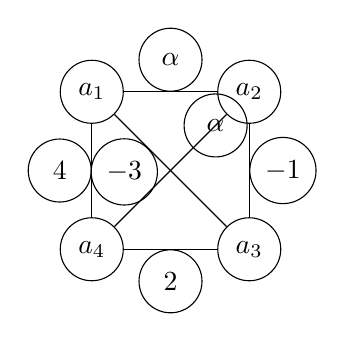
\begin{tikzpicture}[node distance=2cm, every node/.style={circle, draw, minimum size=0.8cm}]
  \node (a1) {$a_1$};
  \node (a2) [right of=a1] {$a_2$};
  \node (a3) [below of=a2] {$a_3$};
  \node (a4) [below of=a1] {$a_4$};
  \draw (a1) -- node[above] {$\alpha$} (a2);
  \draw (a2) -- node[right] {$-1$} (a3);
  \draw (a3) -- node[below] {$2$} (a4);
  \draw (a1) -- node[left] {$4$} (a4);
  \draw (a2) -- node[above right, pos=0.3] {$\alpha$} (a4);
  \draw (a1) -- node[below left, pos=0.3] {$-3$} (a3);
\end{tikzpicture}
\end{center}

Consider $\text{CS} = \{\{a_1, a_2, a_3\}, \{a_4\}\}$.

\textbf{Step 1: Compute utilities in CS.}
\begin{itemize}
  \item $u_1(\{a_1,a_2,a_3\}) = v_1(a_2) + v_1(a_3) = \alpha + (-3) = \alpha - 3$
  \item $u_2(\{a_1,a_2,a_3\}) = v_2(a_1) + v_2(a_3) = \alpha + (-1) = \alpha - 1$
  \item $u_3(\{a_1,a_2,a_3\}) = v_3(a_1) + v_3(a_2) = -3 + (-1) = -4$
  \item $u_4(\{a_4\}) = 0$
\end{itemize}

\textbf{(a) Individually rational} if every player prefers their coalition to being alone ($u_i(S_i) \geq 0$):
\begin{itemize}
  \item $u_1 = \alpha - 3 \geq 0 \Rightarrow \alpha \geq 3$
  \item $u_2 = \alpha - 1 \geq 0 \Rightarrow \alpha \geq 1$
  \item $u_3 = -4 < 0$ always!
  \item $u_4 = 0 \geq 0$ always.
\end{itemize}

$\Rightarrow$ CS is \textbf{never individually rational} (agent $a_3$ always prefers being alone).

\textbf{(b) Nash stable} if no player can benefit by moving to another coalition or forming a singleton. Since CS is never IR, it is \textbf{never Nash stable} (Nash stability implies IR).

\textbf{(c) In the core} if no group of players blocks. Since even singleton $\{a_3\}$ blocks (as $a_3$ prefers being alone), CS is \textbf{never in the core}.
\end{exbox}

\begin{exbox}[Worked Example 2: DA Worst-Case Proposals]
\textbf{Problem:} Construct an instance with $n$ men and $n$ women where each man makes at least $n - 1$ proposals under DA.

\textbf{Construction:} Let all men rank women identically: $w_1 \succ w_2 \succ \cdots \succ w_n$. Let woman $w_i$ rank man $m_i$ first (and the rest in any order).

\textbf{Execution:}
\begin{itemize}
  \item \textbf{Round 1:} All $n$ men propose to $w_1$. She accepts $m_1$ (her favourite), rejects $n-1$ men.
  \item \textbf{Round 2:} Rejected men propose to $w_2$. She accepts $m_2$, rejects the rest.
  \item \textbf{Round $k$:} The $n - k + 1$ remaining men propose to $w_k$. She accepts $m_k$.
  \item Man $m_n$ proposes to $w_1, w_2, \ldots, w_n$ (all $n$ proposals). Man $m_1$ proposes once.
\end{itemize}

Man $m_k$ makes $k$ proposals. Total proposals: $1 + 2 + \cdots + n = \frac{n(n+1)}{2} = \Theta(n^2)$.

Each man $m_k$ (for $k \geq 2$) makes at least $k \geq 2$ proposals; man $m_n$ makes $n$ proposals.

To ensure \textbf{each} man makes $\geq n-1$ proposals, modify so that woman $w_i$ ranks man $m_{n-i+1}$ first (reverse order). Then every man proposes to all but one woman before being accepted.
\end{exbox}

\begin{exbox}[Worked Example 3: Uniform Men's Preferences]
\textbf{Problem:} All men rank women in the same order: $w_1 \succ w_2 \succ \cdots \succ w_n$. The $i$-th woman ranks $m_i$ first. Describe the DA outcome.

\textbf{Outcome:} $M = \{w_i\text{--}m_i : 1 \leq i \leq n\}$ (each woman matched to her favourite man).

\textbf{Why:} By the analysis above, the algorithm proceeds round by round. In round $k$, all unmatched men propose to $w_k$. Woman $w_k$ accepts $m_k$ (her top choice) and rejects the rest. After $n$ rounds, $m_i$ is matched to $w_i$.

This is both the man-optimal and women-optimal stable matching (it is the \textbf{unique} stable matching).
\end{exbox}

\bigseparator

% --- Summary Table ---
\subsubsection{Summary: Key Concepts}

\begin{center}
\renewcommand{\arraystretch}{1.4}
\begin{tabular}{@{} l p{9.5cm} @{}}
\toprule
\textbf{Concept} & \textbf{Key Fact} \\
\midrule
NTU game & Payoffs to individuals, not transferable; must track payoff vectors \\
Hedonic game & Player's utility depends only on coalition membership; outcome is a partition \\
ASHG & $v_i(S) = \sum_{j \in S \setminus \{i\}} v_i(j)$; directed graph representation \\
Nash stability & No unilateral move to another coalition; exists for symmetric ASHGs \\
CIS & Deviation needs approval from both joining and leaving coalitions; always exists \\
Core stability & No group can jointly deviate; may be empty even in symmetric ASHGs \\
Stable matching & Perfect matching with no blocking pairs \\
DA algorithm & $O(n^2)$, always finds stable matching; man-optimal, women-pessimal \\
Strategyproof & DA is strategyproof for proposers only \\
Stable roommates & One-sided variant; stable matching may not exist \\
\bottomrule
\end{tabular}
\end{center}
